% =====================================================================
%  Chapitre 4 -- Classification et evaluation
%  Partie a : regression logistique, seuil, matrice de confusion
% =====================================================================
\section{Chapitre 4 --- Classification et évaluation}

\chapterslide{Chapitre 4}{Classification et évaluation}%
{8 h --- 5 h CM/TD + 3 h TP}%
{\textbf{Objectifs.} Construire un classifieur probabiliste ; choisir un seuil ;
lire une matrice de confusion ; distinguer précision, rappel et $F_1$ ; évaluer
sans se tromper sur des classes déséquilibrées.}

\begin{frame}{Prédire une classe, et surtout une probabilité}
\begin{columns}[t]
\begin{column}{0.48\textwidth}
\begin{ebox}[La sortie]
Une étiquette $\hat y\in\{0,1\}$, mais aussi la \textbf{probabilité}
$\hat p=P(y=1\mid x)$ qui permet de décider \emph{autrement} qu'à 0,5.
\end{ebox}
\end{column}
\begin{column}{0.48\textwidth}
\begin{kbox}[Pourquoi la probabilité compte]
Un tri médical, un contrôle antifraude ou un filtre de courriel n'ont pas le
même coût d'erreur. La probabilité permet d'adapter la décision au coût.
\end{kbox}
\end{column}
\end{columns}
\vspace{2mm}
\begin{solbox}[Le modèle de référence]
La \textbf{régression logistique} : un score linéaire, transformé en probabilité
par la fonction sigmoïde.
\end{solbox}
\end{frame}

\begin{frame}{Du score linéaire à la probabilité}
\begin{columns}[t]
\begin{column}{0.50\textwidth}
\centering
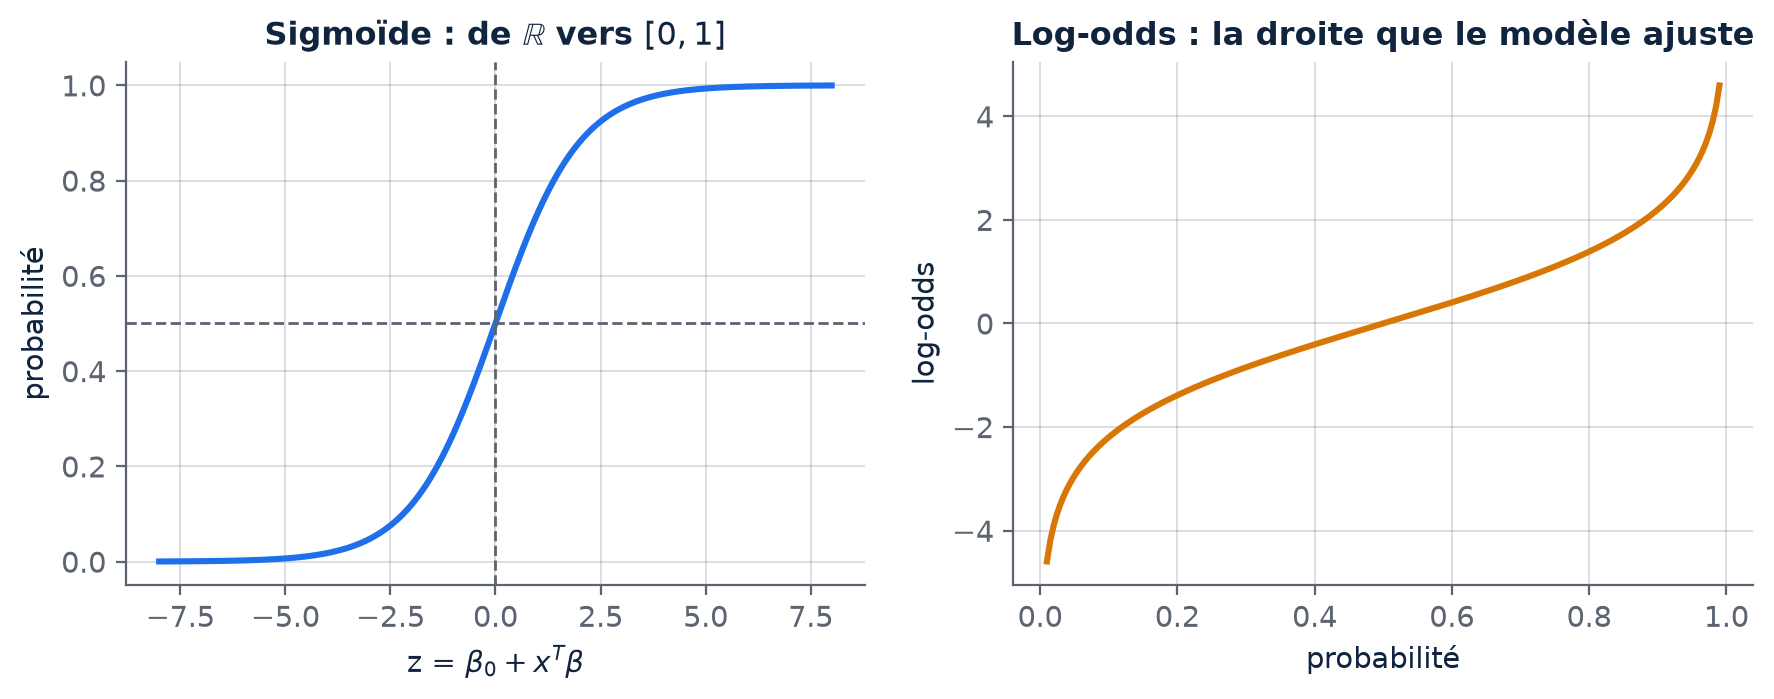
\includegraphics[height=0.30\textheight,keepaspectratio]{l01_sigmoide.png}
\end{column}
\begin{column}{0.46\textwidth}
\[
  z=\beta_0+\mathbf{x}^\top\boldsymbol\beta,
  \qquad
  \hat p=\sigma(z)=\frac{1}{1+e^{-z}} .
\]
\begin{itemize}
  \item $z=0$ $\rightarrow$ $\hat p=0{,}5$.
  \item $z\to+\infty$ $\rightarrow$ $\hat p\to1$.
  \item La frontière est la droite $z=0$.
\end{itemize}
\end{column}
\end{columns}
\vspace{1mm}
\begin{kbox}[Le log-odds]
$\ln\frac{p}{1-p}=z$ : le modèle est \textbf{linéaire en log-odds}, pas en
probabilité. Un coefficient de $0{,}7$ multiplie les cotes par $e^{0,7}\approx2$.
\end{kbox}
\end{frame}

\begin{frame}{La fonction de coût : entropie croisée}
\begin{columns}[t]
\begin{column}{0.50\textwidth}
\[
  L=-\frac1n\sum_{i=1}^{n}\Big[y_i\ln\hat p_i+(1-y_i)\ln(1-\hat p_i)\Big]
\]
\begin{itemize}
  \item $y=1$ et $\hat p=0{,}99$ : coût $\approx0{,}01$.
  \item $y=1$ et $\hat p=0{,}01$ : coût $\approx4{,}6$.
\end{itemize}
\end{column}
\begin{column}{0.46\textwidth}
\begin{kbox}[Pourquoi pas les moindres carrés ?]
Avec la sigmoïde, la perte quadratique n'est pas convexe : l'optimisation peut
rester bloquée. L'entropie croisée l'est.
\end{kbox}
\begin{wbox}[Le lien avec la vraisemblance]
Minimiser l'entropie croisée, c'est maximiser la vraisemblance des étiquettes
observées.
\end{wbox}
\end{column}
\end{columns}
\end{frame}

\begin{frame}{La frontière de décision}
\begin{columns}[t]
\begin{column}{0.48\textwidth}
\centering
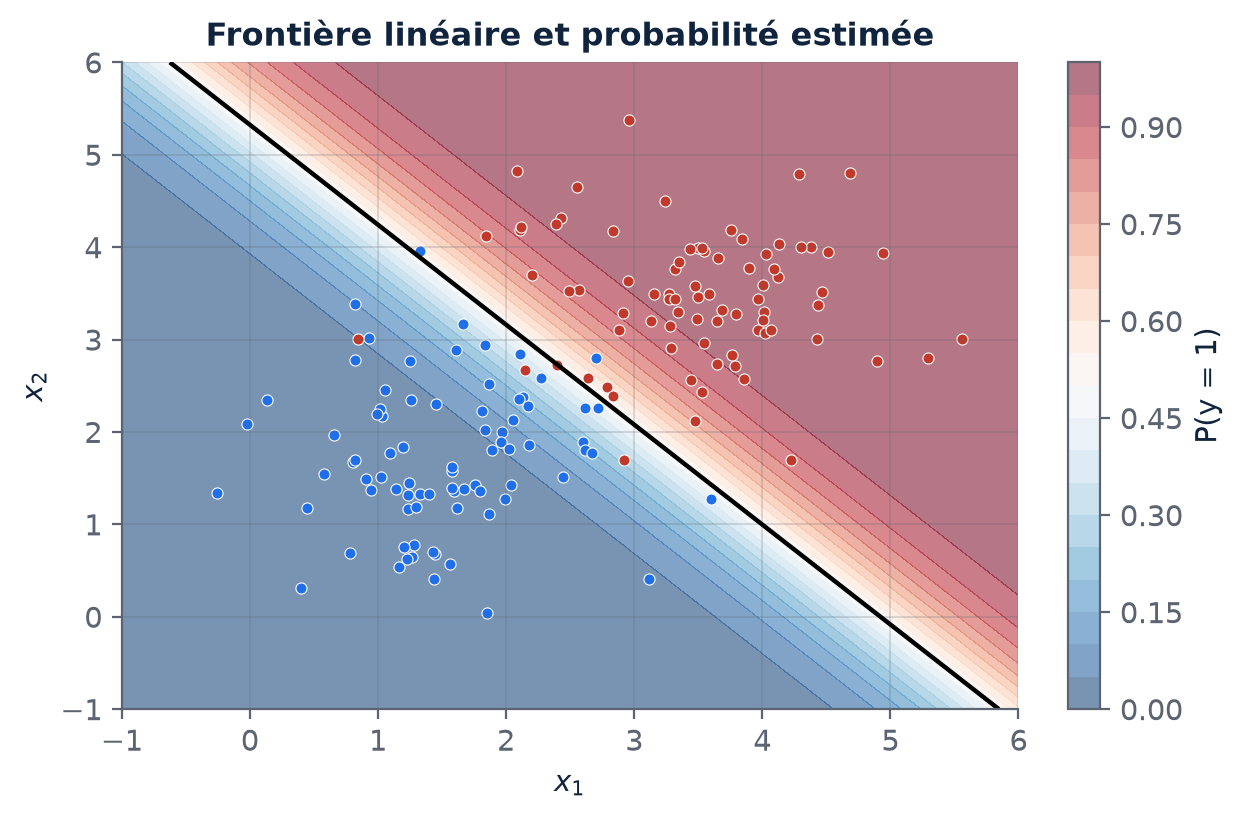
\includegraphics[height=0.34\textheight,keepaspectratio]{l02_frontiere.png}
\end{column}
\begin{column}{0.48\textwidth}
\begin{itemize}
  \item La couleur est la probabilité estimée.
  \item La ligne noire est l'ensemble des points où $\hat p=0{,}5$.
  \item Un modèle linéaire ne peut pas produire une frontière courbe : pour
        cela, il faut ajouter des variables polynomiales ou changer de modèle.
\end{itemize}
\begin{wbox}[Le seuil déplace la frontière]
Décider à 0,3 au lieu de 0,5 déplace la ligne vers la classe négative.
\end{wbox}
\end{column}
\end{columns}
\end{frame}

\begin{frame}{Un classifieur, six nombres}
\begin{columns}[t]
\begin{column}{0.44\textwidth}
\centering
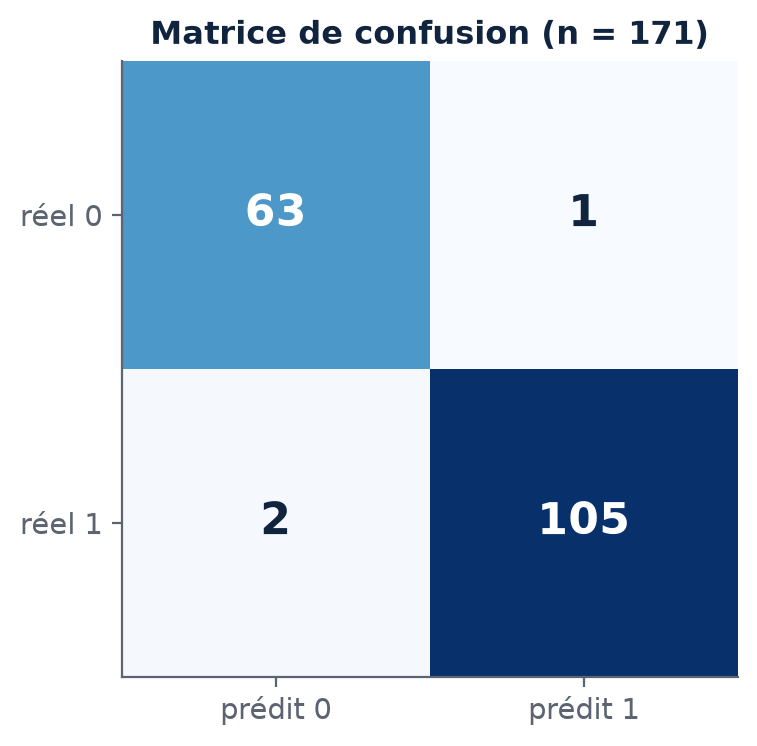
\includegraphics[height=0.25\textheight,keepaspectratio]{l03_matrice.png}
\end{column}
\begin{column}{0.54\textwidth}
\begin{center}
\small
\begin{tabular}{@{}ll@{}}
\toprule
\textbf{Nom} & \textbf{Définition} \\
\midrule
Exactitude & $\dfrac{VP+VN}{n}$ \\
Précision & $\dfrac{VP}{VP+FP}$ \\
Rappel (sensibilité) & $\dfrac{VP}{VP+FN}$ \\
Spécificité & $\dfrac{VN}{VN+FP}$ \\
$F_1$ & $2\cdot\dfrac{P\cdot R}{P+R}$ \\
\bottomrule
\end{tabular}
\end{center}
\end{column}
\end{columns}
\vspace{1mm}
\begin{kbox}[Sur le cancer du sein : $VP=105$, $VN=63$, $FP=1$, $FN=2$]
Exactitude $0{,}9825$ · précision $0{,}9906$ · rappel $0{,}9813$ · $F_1$ $0{,}9859$.
\end{kbox}
\end{frame}

\begin{frame}{Lire les coefficients en cotes}
\begin{columns}[t]
\begin{column}{0.50\textwidth}
Le modèle est linéaire en log-odds :
\[
  \ln\frac{\hat p}{1-\hat p}=\beta_0+\beta_1x_1+\dots
\]
Donc
\[
  \frac{\text{cote}(x_j+1)}{\text{cote}(x_j)}=e^{\beta_j}.
\]
\end{column}
\begin{column}{0.46\textwidth}
\begin{center}
\small
\begin{tabular}{@{}rr@{}}
\toprule
$\beta_j$ & $e^{\beta_j}$ \\
\midrule
$0{,}00$ & $1{,}00$ \\
$0{,}69$ & $2{,}00$ \\
$1{,}10$ & $3{,}00$ \\
$-0{,}69$ & $0{,}50$ \\
\bottomrule
\end{tabular}
\end{center}
\end{column}
\end{columns}
\vspace{2mm}
\begin{kbox}[La phrase correcte]
« Une unité de plus sur $x_j$ multiplie la cote d'appartenir à la classe 1 par
$e^{\beta_j}$, toutes choses égales. » Pas « augmente la probabilité de
$\beta_j$ » : la probabilité n'est pas linéaire.
\end{kbox}
\end{frame}

\begin{frame}{Sensibilité et spécificité : un curseur}
\begin{columns}[t]
\begin{column}{0.48\textwidth}
\begin{ebox}[Deux taux qui se déplacent en sens inverse]
En baissant le seuil, la \textbf{sensibilité} (rappel) monte et la
\textbf{spécificité} baisse. On ne peut pas maximiser les deux.
\end{ebox}
\end{column}
\begin{column}{0.48\textwidth}
\begin{kbox}[Le point de fonctionnement]
C'est le couple (sensibilité, spécificité) au seuil retenu. Un modèle se juge
\emph{à ce point}, pas dans l'absolu.
\end{kbox}
\end{column}
\end{columns}
\vspace{2mm}
\begin{center}
\small
\begin{tabular}{@{}lrrr@{}}
\toprule
\textbf{Seuil} & \textbf{Sensibilité} & \textbf{Spécificité} & \textbf{Fausses alertes / 1\,000} \\
\midrule
$0{,}5$ & $0{,}981$ & $0{,}984$ & $16$ \\
$0{,}3$ & $1{,}000$ & $0{,}969$ & $31$ \\
$0{,}1$ & $1{,}000$ & $0{,}906$ & $94$ \\
\bottomrule
\end{tabular}
\end{center}
\end{frame}

\begin{frame}{Précision ou rappel : ce n'est pas un choix technique}
\begin{columns}[t]
\begin{column}{0.48\textwidth}
\begin{ebox}[Précision]
Parmi les alertes déclenchées, combien sont justes ?

\vspace{1mm}
Prioritaire quand un faux positif coûte cher : blocage d'un client légitime,
examen médical invasif inutile.
\end{ebox}
\end{column}
\begin{column}{0.48\textwidth}
\begin{ebox}[Rappel]
Parmi les cas réels, combien sont détectés ?

\vspace{1mm}
Prioritaire quand un faux négatif coûte cher : tumeur manquée, fraude non
détectée.
\end{ebox}
\end{column}
\end{columns}
\vspace{2mm}
\begin{wbox}[Le $F_1$ ne tranche pas]
C'est une moyenne harmonique : elle traite les deux erreurs comme également
coûteuses. Si les coûts diffèrent, le $F_1$ n'est pas la bonne métrique.
\end{wbox}
\end{frame}

\begin{frame}{Le seuil est une décision, pas un paramètre par défaut}
\begin{columns}[t]
\begin{column}{0.52\textwidth}
\centering
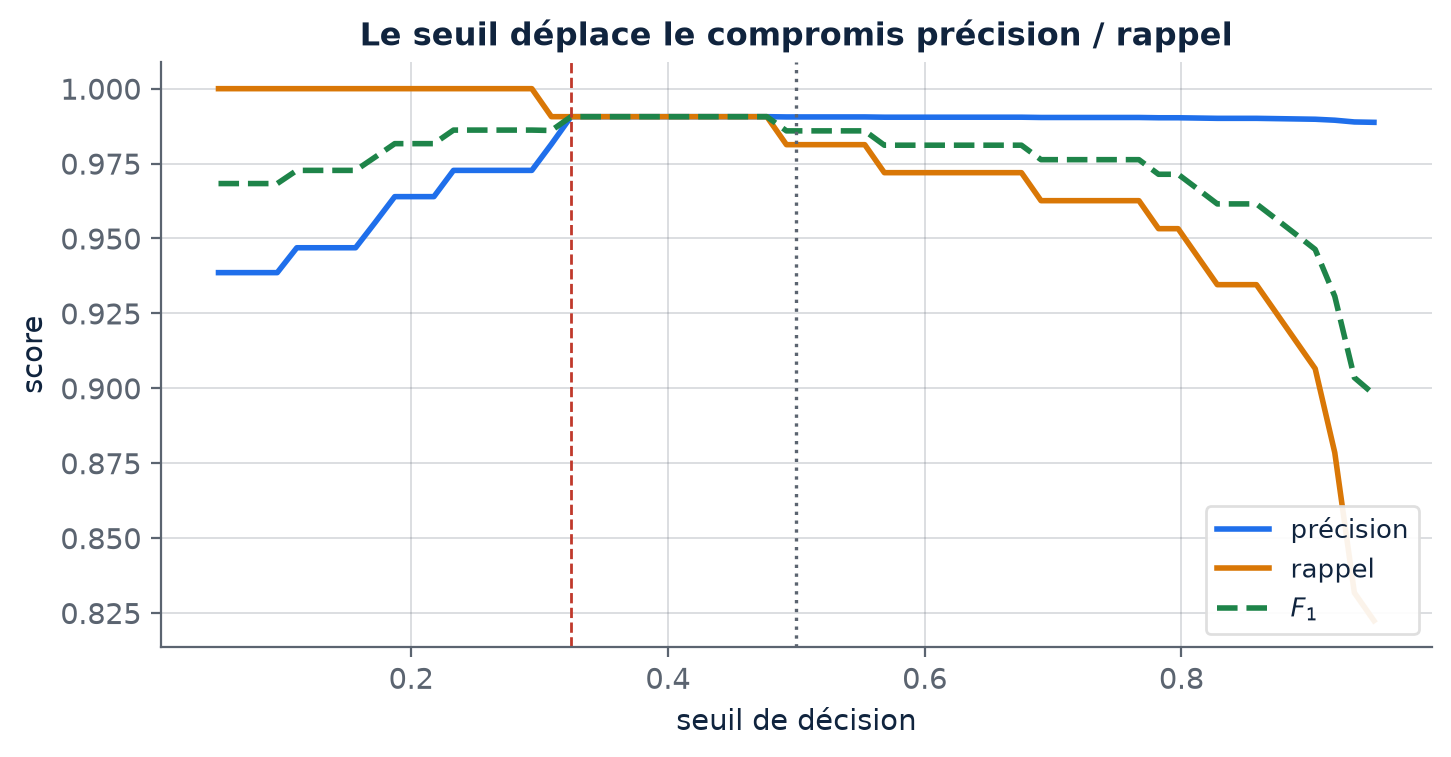
\includegraphics[height=0.30\textheight,keepaspectratio]{l04_seuil.png}
\end{column}
\begin{column}{0.44\textwidth}
\begin{itemize}
  \item À 0,5 : précision $0{,}991$, rappel $0{,}981$.
  \item Le $F_1$ maximal est atteint à $\mathbf{0{,}325}$ ($F_1=0{,}991$).
  \item Descendre le seuil augmente le rappel et diminue la précision.
\end{itemize}
\end{column}
\end{columns}
\vspace{1mm}
\begin{kbox}[À retenir]
Le seuil se choisit selon le \textbf{coût des erreurs}, sur des données de
validation — jamais sur le test.
\end{kbox}
\end{frame}

\begin{frame}{Le seuil par le coût : le calcul qui décide}
\begin{columns}[t]
\begin{column}{0.50\textwidth}
Soit $C_{FP}$ le coût d'une fausse alerte et $C_{FN}$ celui d'un cas manqué.
On déclenche si :
\[
  \hat p \;>\; \frac{C_{FP}}{C_{FP}+C_{FN}} .
\]
\begin{itemize}
  \item $C_{FP}=C_{FN}$ $\rightarrow$ seuil $0{,}5$.
  \item $C_{FN}=10\,C_{FP}$ $\rightarrow$ seuil $1/11\approx0{,}091$.
\end{itemize}
\end{column}
\begin{column}{0.46\textwidth}
\begin{kbox}[Lecture]
Plus un cas manqué est grave, plus on abaisse le seuil : on accepte davantage
de fausses alertes pour ne rien laisser passer.
\end{kbox}
\begin{wbox}[Le piège]
Ce calcul suppose des probabilités \textbf{calibrées}. Un modèle qui annonce
0,9 alors qu'il a raison 60 \% du temps fausse tout le raisonnement.
\end{wbox}
\end{column}
\end{columns}
\end{frame}

\begin{frame}{Activité 1 --- lire une matrice (10 min)}
\begin{abox}[Dépistage sur 1\,000 personnes]
$VP=48$, $FN=12$, $FP=90$, $VN=850$.
\begin{enumerate}
  \item Calculer exactitude, précision, rappel, spécificité.
  \item Que dire à un médecin qui ne regarde que l'exactitude ?
  \item Quel seuil choisir si manquer un cas est jugé dix fois plus grave
        qu'une fausse alerte ?
\end{enumerate}
\end{abox}
\vspace{1mm}
\begin{solbox}[Réponses]
\textbf{1.} Exactitude $898/1000=0{,}898$ ; précision $48/138=0{,}348$ ;
rappel $48/60=0{,}80$ ; spécificité $850/940=0{,}904$.\\
\textbf{2.} 89,8 \% masque que 2 alertes sur 3 sont fausses.\\
\textbf{3.} Seuil $1/11\approx0{,}09$, ce qui augmentera le rappel et les fausses alertes.
\end{solbox}
\end{frame}

\begin{frame}{Quiz 1 --- vocabulaire}
\begin{columns}[t]
\begin{column}{0.49\textwidth}
\begin{qbox}[Question 1]
Le rappel mesure :
\begin{itemize}
  \item[(a)] la part de positifs bien détectés
  \item[(b)] la part d'alertes justes
  \item[(c)] l'exactitude
\end{itemize}
\end{qbox}
\begin{qbox}[Question 2]
Baisser le seuil :
\begin{itemize}
  \item[(a)] augmente le rappel
  \item[(b)] augmente la précision
  \item[(c)] ne change rien
\end{itemize}
\end{qbox}
\end{column}
\begin{column}{0.49\textwidth}
\begin{qbox}[Question 3]
Le $F_1$ est la moyenne :
\begin{itemize}
  \item[(a)] arithmétique \quad (b) harmonique
  \item[(c)] géométrique
\end{itemize}
\end{qbox}
\begin{solbox}[Réponses]
\textbf{1.} (a). \quad \textbf{2.} (a). \quad \textbf{3.} (b), ce qui pénalise
les cas où l'une des deux est faible.
\end{solbox}
\end{column}
\end{columns}
\end{frame}
